%\section {Collision tests}

%
%  Collision tests
%
\begin{frame} {Collision tests}
  \begin{itemize}
  \item for configurations
    \begin{itemize}
    \item problem: given
      \begin{itemize}
      \item two rigid sets of triangles,
      \item the relative position of one set with respect to the other set,
      \end{itemize}
      determine whether the intersection between the sets is empty, or compute
      the distance between the sets.
    \end{itemize}
  \end{itemize}
\end{frame}

%
%  Hierarchy of bounding volumes
%
\begin{frame} {Hierarchy of bounding volumes}
  \begin{itemize}
  \item Binary trees of bounding volumes such that
    \begin{itemize}
    \item each node contains two children,
    \item leaves are the triangles
    \end{itemize}
  \end{itemize}
  \centerline {
    \includegraphics[width=.8\linewidth]{figures/bvh1.pdf}
  }
\end{frame}

\begin{frame} {Hierarchy of bounding volumes}
  \begin{itemize}
  \item Binary trees of bounding volumes such that
    \begin{itemize}
    \item each node contains two children,
    \item leaves are the triangles
    \end{itemize}
  \end{itemize}
  \centerline {
    \includegraphics[width=.8\linewidth]{figures/bvh2.pdf}
  }
\end{frame}

\begin{frame} {Hierarchy of bounding volumes}
  \begin{itemize}
  \item Binary trees of bounding volumes such that
    \begin{itemize}
    \item each node contains two children,
    \item leaves are the triangles
    \end{itemize}
  \end{itemize}
  \centerline {
    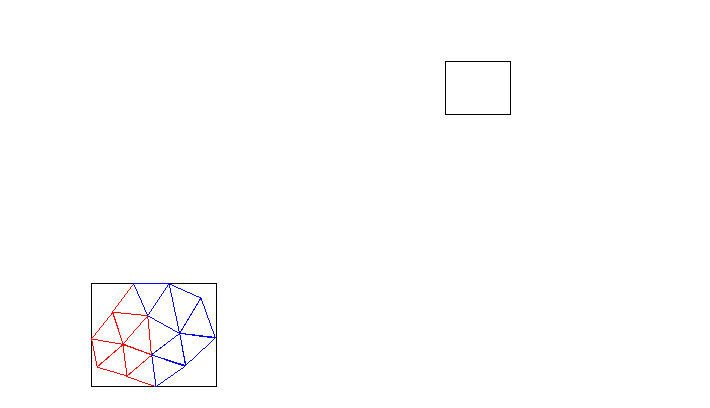
\includegraphics[width=.8\linewidth]{figures/bvh3.pdf}
  }
\end{frame}

\begin{frame} {Hierarchy of bounding volumes}
  \begin{itemize}
  \item Binary trees of bounding volumes such that
    \begin{itemize}
    \item each node contains two children,
    \item leaves are the triangles
    \end{itemize}
  \end{itemize}
  \centerline {
    \includegraphics[width=.8\linewidth]{figures/bvh4.pdf}
  }
\end{frame}

\begin{frame} {Hierarchy of bounding volumes}
  \begin{itemize}
  \item Binary trees of bounding volumes such that
    \begin{itemize}
    \item each node contains two children,
    \item leaves are the triangles
    \end{itemize}
  \end{itemize}
  \centerline {
    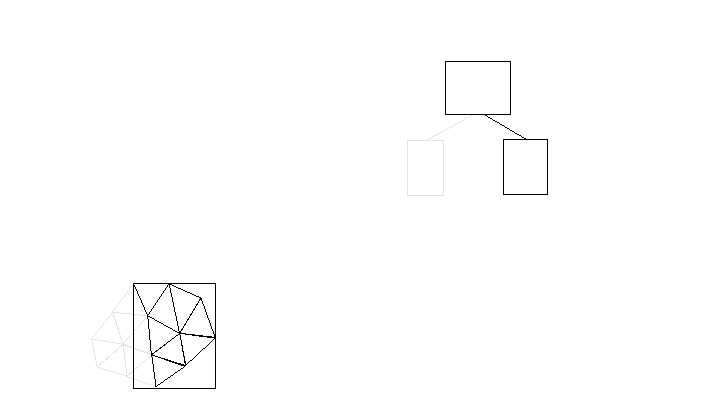
\includegraphics[width=.8\linewidth]{figures/bvh5.pdf}
  }
\end{frame}

\begin{frame} {Hierarchy of bounding volumes}
  \begin{itemize}
  \item Binary trees of bounding volumes such that
    \begin{itemize}
    \item each node contains two children,
    \item leaves are the triangles
    \end{itemize}
  \end{itemize}
  \centerline {
    \includegraphics[width=.8\linewidth]{figures/bvh6.pdf}
  }
\end{frame}

\begin{frame} {Hierarchy of bounding volumes}
  \begin{itemize}
  \item Binary trees of bounding volumes such that
    \begin{itemize}
    \item each node contains two children,
    \item leaves are the triangles
    \end{itemize}
  \end{itemize}
  \centerline {
    \includegraphics[width=.8\linewidth]{figures/bvh7.pdf}
  }
\end{frame}

\begin{frame} {Hierarchy of bounding volumes}
  \begin{itemize}
  \item Binary trees of bounding volumes such that
    \begin{itemize}
    \item each node contains two children,
    \item leaves are the triangles
    \end{itemize}
  \end{itemize}
  \centerline {
    \includegraphics[width=.8\linewidth]{figures/bvh8.pdf}
  }
\end{frame}

\begin{frame} {Hierarchy of bounding volumes}
  \begin{itemize}
  \item Binary trees of bounding volumes such that
    \begin{itemize}
    \item each node contains two children,
    \item leaves are the triangles
    \end{itemize}
  \end{itemize}
  \centerline {
    \includegraphics[width=.8\linewidth]{figures/bvh9.pdf}
  }
\end{frame}

%
%  Collision tests for configurations
%

\begin{frame} {Collision tests for configurations}
  \begin{itemize}
  \item Algorithm
    \begin{itemize}
    \item test root nodes of each tree against one another
    \item if two nodes are in collision, test one with the children of the other node
    \end{itemize}
    \centerline {
      \includegraphics[width=.8\linewidth]{figures/collision-test1.pdf}
    }
  \end{itemize}

\end{frame}

\begin{frame} {Collision tests for configurations}
  \begin{itemize}
  \item Algorithm
    \begin{itemize}
    \item test root nodes of each tree against one another
    \item if two nodes are in collision, test one with the children of the other node
    \end{itemize}
    \centerline {
      \includegraphics[width=.8\linewidth]{figures/collision-test2.pdf}
    }
  \end{itemize}

\end{frame}

\begin{frame} {Collision tests for configurations}
  \begin{itemize}
  \item Algorithm
    \begin{itemize}
    \item test root nodes of each tree against one another
    \item if two nodes are in collision, test one with the children of the other node
    \end{itemize}
    \centerline {
      \includegraphics[width=.8\linewidth]{figures/collision-test3.pdf}
    }
  \end{itemize}

\end{frame}

\begin{frame} {Collision tests for configurations}
  \begin{itemize}
  \item Algorithm
    \begin{itemize}
    \item test root nodes of each tree against one another
    \item if two nodes are in collision, test one with the children of the other node
    \end{itemize}
    \centerline {
      \includegraphics[width=.8\linewidth]{figures/collision-test4.pdf}
    }
  \end{itemize}

\end{frame}
